\documentclass{article}
\usepackage[spanish]{babel}
\usepackage[a4paper,top=2cm,bottom=2cm,left=3cm,right=3cm,marginparwidth=1.75cm]{geometry}
\usepackage{amsmath}
\usepackage{graphicx}
\usepackage{float}
\usepackage[colorlinks=true, allcolors=blue]{hyperref}
\hypersetup{linkcolor=black}

\title{Certificación Profesional en Python (ITBA) \\
Trabajo Práctico Final\\
Manual de usuario}
\author{Matías Huenul}
\date{}
\begin{document}
\maketitle
\tableofcontents
\newpage

\section{Requisitos}
El programa requiere \textbf{matplotlib} para realizar los
gráficos. Se puede instalar con \textbf{pip} corriendo el siguiente comando.
\begin{figure}[H]
\centering

\includegraphics[width=0.9\textwidth]{img/instalacion_matplotlib.png}
\end{figure}

\section{Configuración}
Antes de ejecutar el programa se debe crear la \textbf{variable de entorno}
que almacenará la clave provista por Polygon. En Linux o Git Bash, se puede
correr el siguiente comando, ingresando la clave correspondiente.
\begin{figure}[H]
\centering

\includegraphics[width=0.9\textwidth]{img/configuracion_api_key.png}
\end{figure}

\section{Uso}
El programa se ejecuta por línea de comandos. Para esto se debe posicionar
dentro de la carpeta \textbf{src} y correr el script \textbf{main.py} de la
siguiente forma.
\begin{figure}[H]
\centering

\includegraphics[width=0.9\textwidth]{img/ejecucion_del_programa.png}
\end{figure}

\subsection{Actualizar datos}
\begin{figure}[H]
\centering
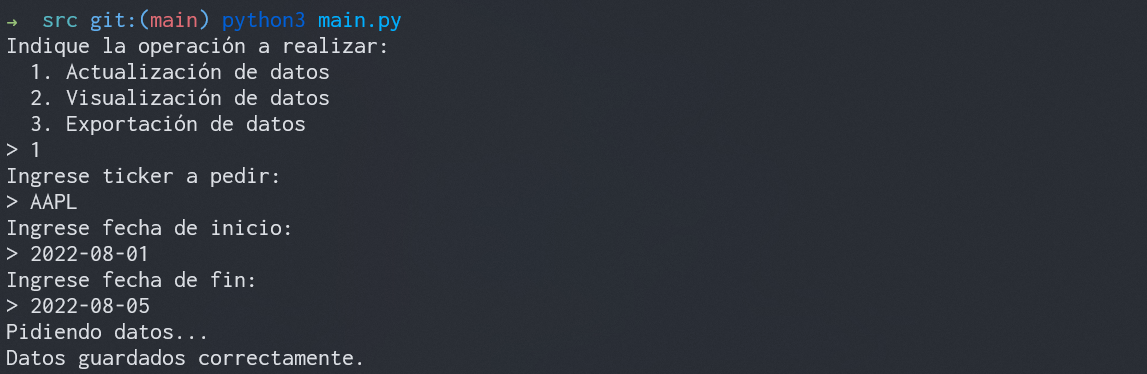
\includegraphics[width=0.9\textwidth]{img/actualizacion_de_datos.png}
\end{figure}

\subsection{Obtener resumen de datos}

\begin{figure}[H]
\centering
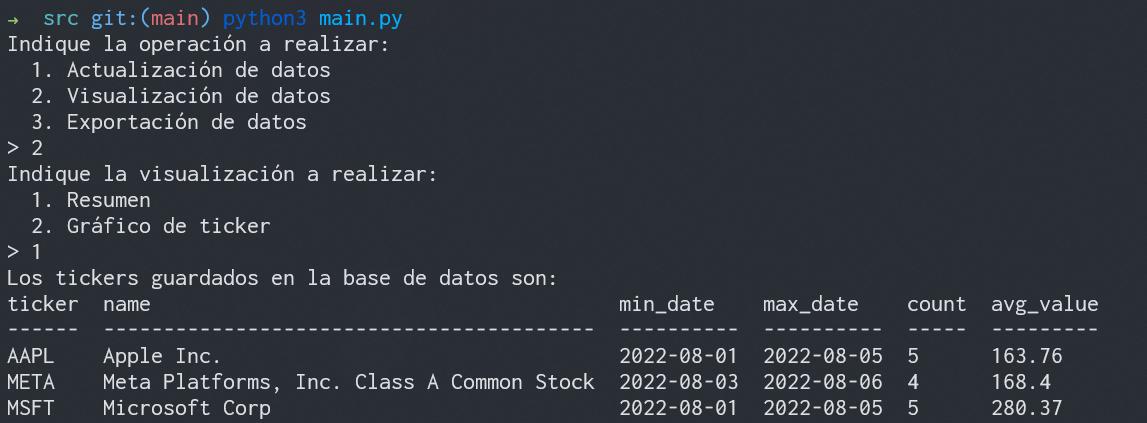
\includegraphics[width=0.9\textwidth]{img/visualizacion_resumen.png}
\end{figure}

\subsection{Graficar valor de ticker}
\begin{figure}[H]
\centering
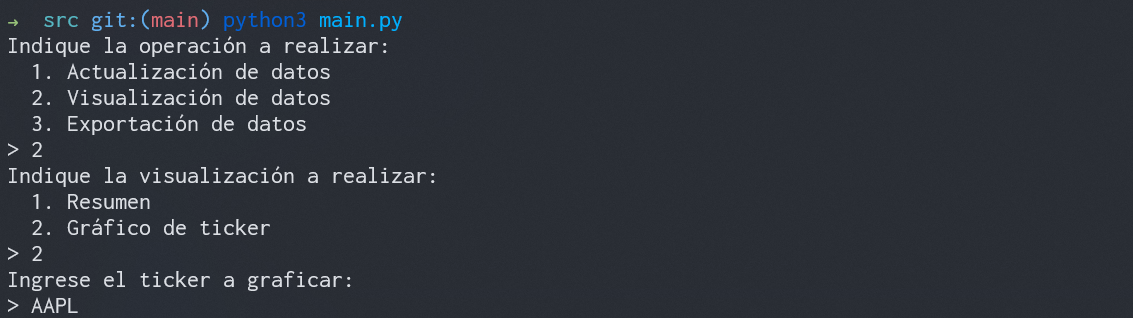
\includegraphics[width=0.9\textwidth]{img/visualizacion_grafico_1.png}
\end{figure}

\begin{figure}[H]
\centering
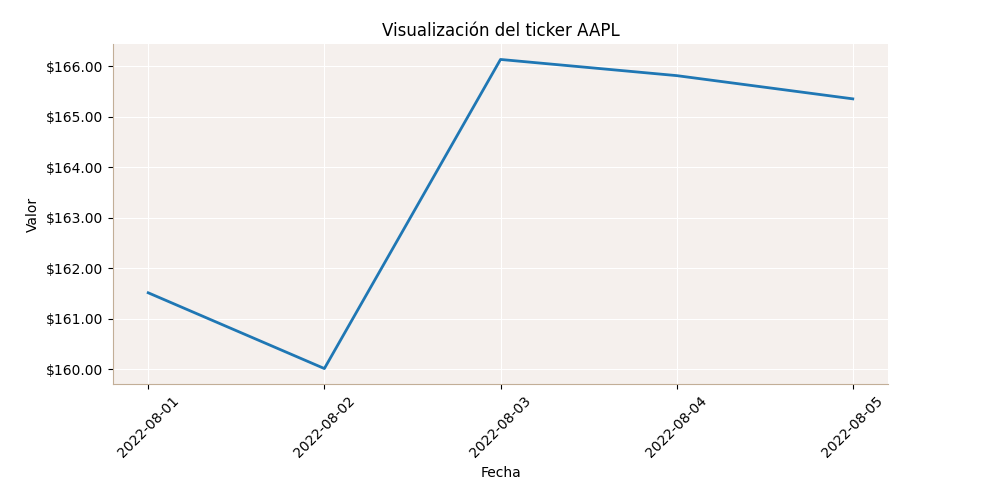
\includegraphics[width=0.9\textwidth]{img/visualizacion_grafico_2.png}
\end{figure}

\subsection{Exportar datos}
\begin{figure}[H]
\centering
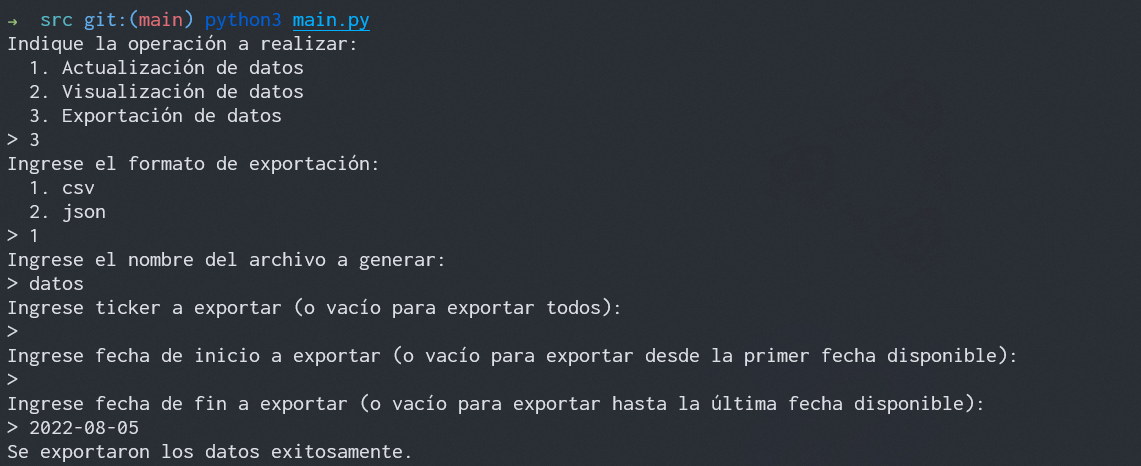
\includegraphics[width=0.9\textwidth]{img/exportacion_de_datos_1.png}
\end{figure}

\begin{figure}[H]
\centering
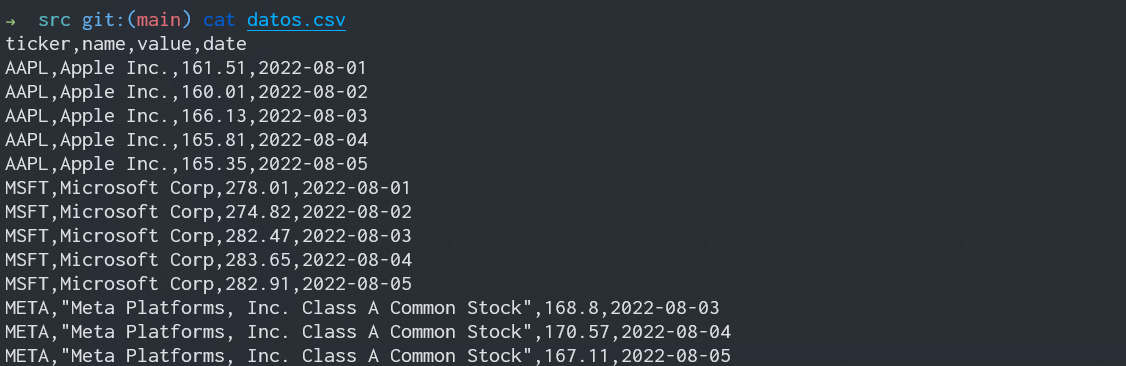
\includegraphics[width=0.9\textwidth]{img/exportacion_de_datos_2.png}
\end{figure}

\end{document}
